% getting_started.tex

\chapter{Getting Started}
This chapter provides a short real-world example of performing symbolic regression with \RGP.

\section{Installation}

The newest release version of \RGP is always available on CRAN. To install it just type
\lstinline!install.packages(``rgp'')! 

\section{Problem Definition}

For a first run of \RGP you need to define a fitting problem.
\begin{lstlisting}[caption = {Creating a function with variables}, label = lstExample]
makeDampedPendulum <- function(A0 = 1, g = 9.81, l = 0.1, phi = pi, gamma = 0.5) {
  omega <- sqrt(g/l)
  function(t) A0 * exp(-gamma * t) * cos(omega * t + phi)
}
\end{lstlisting}

The function above represents a damped mathematical Pendulum, the arguments are the starting Amplitude A0, 
gravity g, length of pendulum l, phase, radial frequency omega and damping gamma.

\begin{lstlisting}[caption = {Attributes}, label = tutattributes]
dampedPendulum1 <- makeDampedPendulum(l = 0.5)
\end{lstlisting}

Here is a example of alternating the given attributes, 
the lenght is altered and the function is assigned to a new name.

With \lstinline!xs1 <- seq(from=1, to=10, length.out=512)!
a list of numbers is definded for creating a dataframe. It creates a subsequent list of numbers from 1 to 10
with 512 steps.

\begin{lstlisting}[caption = {Data Frame Creation}, label = tutdataframe]
dampedPendulumData <- data.frame(time=xs1,
  amplitude=dampedPendulum1(xs1) + rnorm(length(xs1), sd=0.01))
\end{lstlisting}

We create a time series dataframe with the sequence defined above. 
The dataframe consists of the sequence xs1 as time, the amplitude defined through our pendulum-function and a
interference function.
To plot the prepared data frame type \lstinline!plot(dampedPendulumData, pch=20)!.

Now let's shift attention to the more interesting objects.
First, we need to activate \RGP using \lstinline!require(rgp)!.
We are going to perform a symbolic regression with our pendulum data.
The time permitted for the regression are 2 minutes ( 2 * 60 seconds ).
To start the symbolic regression you need the following code.

\begin{lstlisting}[caption = {Symbolic Regression }, label = tutsymbolicregression]
modelSet1 <- symbolicRegression(amplitude ~ time, data=dampedPendulumData,
                                stopCondition=makeTimeStopCondition(2 * 60))
\end{lstlisting}

Now we got a set of models with variable fitness. 
To get our desired prediction we are going to use the model with the best training fitness
which gives the best results.

\begin{lstlisting}[caption = {Best Model}, label = tutbestmodel]
bestModel1 <- modelSet1$population[[which.min(Map(modelSet1$fitnessFunction, 
  modelSet1$population))]]

bestModel1
\end{lstlisting}

Let's start the prediction and plot our given and predicted data. 

\begin{lstlisting}[caption = {Prediction}, label = tutPrediction]

predictedData <- data.frame(time=xs1,
  amplitude=predict(modelSet1, newdata=dampedPendulumData))

#plot data
plot(dampedPendulumData, pch=20)
points(predictedData, pch=20, col=2)

\end{lstlisting}

The plot shows the difference between the real and the predicted data. 
As you see, the outcome is not ideal. To get better results we need to extend the processing time.

\begin{figure*}[h]
  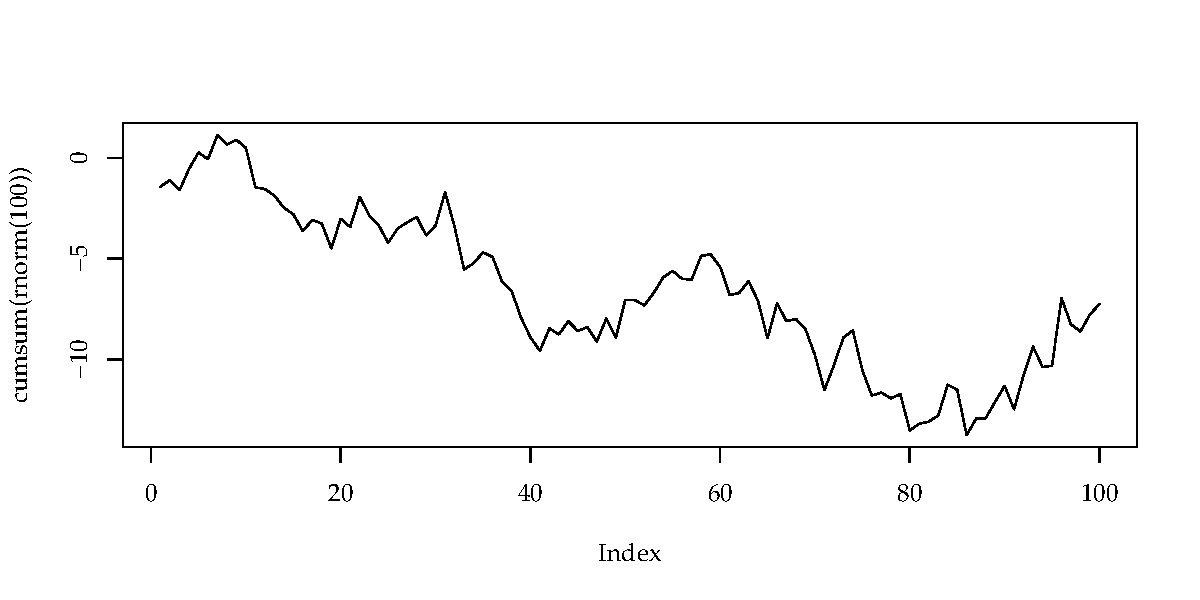
\includegraphics[width=\linewidth]{getting_started/test.pdf}
  \caption{This figure shows how to add figures to \LaTeX documents.}
  \label{fig:test}
  \setfloatalignment{t}
\end{figure*}
